\documentclass{unimapcgsfyp}
%%%%%%%%%%%%%%%%%%%%%%%%%%%%%%%%%%%%%%%%%%%%%%%%%%%%%%%
% This is unimapthesis.tex, January 2019.
% Created by Mohd Hanafi Mat Som (DE)
% mhanafi@unimap.edu.my
% http://mohdhanafi.unimap.edu.my/template
%
% This is the "main" file for the thesis,
% formatted according to the Template
% Thesis, published by CGS UniMAP 2018.
%%%%%%%%%%%%%%%%%%%%%%%%%%%%%%%%%%%%%%%%%%%%%%%%%%%%%%%

%% Declare graphics path 
\graphicspath{{./Figures/}}	% a subfolder named figs

%% To SPEED UP compilation, enable this option.
%% This package will replace your figure with textbox but maintain the figure size
%
%\usepackage[allfiguresdraft]{draftfigure}

%% you can opt to show specific chapter for FASTER compilation of the document. 
%% Useful during drafting the thesis.
%% http://web.science.mq.edu.au/~rdale/resources/writingnotes/latexstruct.html
%
%\includeonly{chap-review,chap-design}

%% The enumitem package is great for customising
%% list environments.
\usepackage{enumitem}

%% Listings is a nice package for typesetting code
%% listings. Other possible packages include fancyvrb,
%% minted, etc.
\usepackage{listings}
\lstset{basicstyle=\ttfamily,breaklines=true}

%% Indent first paragraph after section header
\usepackage{indentfirst}

%%%%%%%%%%%%%%%%%%%%%%%%%%%%%%%%%%%%%%%%%%%%%%
%TODO Particulars about your thesis HERE
%%%%%%%%%%%%%%%%%%%%%%%%%%%%%%%%%%%%%%%%%%%%%%
% Your Name
\author{Budin Bin Buyung}
% Your Matric Number
\matric{161150042}
% Your IC/Passport Number
\icpass{201020-89-0089}
% Your Date of Birth
\dob{20 October 2000}
% Your Enrolled School
\schoolname{School of Mechatronic Engineering}
% Your Enrolled Program
%\programname{Biomedical Electronic Engineering}
%% Your Supervisor name
%\supervisor{Dr. Mohd Hanafi Mat Som}
%% Panel 1
%\panelone{Dr. Charles Xavier}
%% Panel 2
%\paneltwo{Dr. Muhammad Juhairi Aziz Safar}
%\paneltwo{Dr. Putri Intan Payung Indah Zulaikha Odelia Ladasyia Absyari}
% English title of your thesis
\title{Writing Your Thesis with LaTeX and It's A Very Long Title That It Span to Three Lines Where the Longer the Title Makes Your Thesis Looks Awesome}
% Malay title of your thesis
\titlems{Menulis Thesis Anda dengan LaTeX dan Ia Merupakan Satu Tajuk yang Sangat Panjang Merangkumi Tiga Baris Dimana Semakin Panjang Tajuk Thesis Menjadikan Thesis Lebih Mengagumkan}
% Academic Session
\acads{2019/2020}
% Year submitted
\submityear{2020}
% Declaration date signed
\declaredate{10 January 2020}
%% Degree name :-)
\degreetype{Bachelor of Engineering (Biomedical Electronic Engineering)} 

%%%%%%%%%%%%%%%%%%%%%%%%%%%%%%%%%%%%%%%%%%%%%%%%%%%%%%%
%TODO List of Publication Header
%  You can comment out the following line if you don't have a
% "List of Own Publications"
%%%%%%%%%%%%%%%%%%%%%%%%%%%%%%%%%%%%%%%%%%%%%%%%%%%%%%%
%\newcites{own}{LIST OF PUBLICATIONS}
%\addbibresource{mybib.bib}

%%%%%%%%%%%%%%%%%%%%%%%%%%%%%%%%%%%%%%%%%%%%%%%%%%%%%%%
% Options for generating hyperlinks when using pdfLaTeX
%%%%%%%%%%%%%%%%%%%%%%%%%%%%%%%%%%%%%%%%%%%%%%%%%%%%%%%
\ifpdf
  \makeatletter
  \usepackage[pdftex,plainpages=false,hypertexnames=false,bookmarksnumbered,pdfpagelabels,%
    pdfauthor={\@author},pdftitle={\@title}]{hyperref}
  \makeatother
\else
  \usepackage[dvips,plainpages=false,bookmarksnumbered,breaklinks=true]{hyperref}
\fi

\usepackage{ragged2e}
%

\begin{document}

%%%%%%%%%%%%%%%%%%%%%%%%%%%%%%%%%%%%%%%%%%%%%%%%%%%%%%%
% Default bibliography style is apa (using 
% \RequirePackage[natbibapa]{apacite} in the class file).
%
% If you prefer the number system though, use bibliography
% style "plainnat" for [1][2][3] or "alpha" for [Jon94] (the label
% will be auto-generated).
%%%%%%%%%%%%%%%%%%%%%%%%%%%%%%%%%%%%%%%%%%%%%%%%%%%%%%%
%\bibliographystyle{apacite}
%\bibliographystyleown{apacite}	% comment this if not using \newcites{own} above
%\bibliographystyle{plainnat}
%\bibliographystyleown{plainnat}
\bibliographystyle{IEEEtranN}

\frontmatter

%%%%%%%%%%%%%%%%%%%%%%%%%%%%%%%%%%%%%%%%%%%%%%%%%%%%%%%
% Inserts the cover page (the hard cover with gold-lettering)
% and the title page 
%%%%%%%%%%%%%%%%%%%%%%%%%%%%%%%%%%%%%%%%%%%%%%%%%%%%%%%
\makecover

%%%%%%%%%%%%%%%%%%%%%%%%%%%%%%%%%%%%%%%%%%%%%%%%%%%%%%%
% TODO Declaration & Panel Approval
%%%%%%%%%%%%%%%%%%%%%%%%%%%%%%%%%%%%%%%%%%%%%%%%%%%%%%%
\declaration
\approval 

%%%%%%%%%%%%%%%%%%%%%%%%%%%%%%%%%%%%%%%%%%%%%%%%%%%%%%%
% MAKE SURE YOU HAVE A acknowledgements.tex FILE
%%%%%%%%%%%%%%%%%%%%%%%%%%%%%%%%%%%%%%%%%%%%%%%%%%%%%%%
\chapter{Acknowledgement}

Many thanks to Prof.~Donald Knuth for giving us \TeX, and Leslie Lamport for \LaTeX.  

I first heard about \LaTeX{} as a postgraduate student in Australia. But back then, I have no idea how the \LaTeX{} works. Then, I started to learn how to \textbf{use} \LaTeX{} for conference/journal paper. I planned to write my Doctor of Engineering (DE) thesis (University of Fukui, Japan) in \LaTeX{} but somehow my supervisor is more comfortable with standard word processor. So, good bye \LaTeX{}!!. 

Back in Malaysia, I picked it up again because I want to make a \LaTeX{} template for postgraduate thesis in UniMAP. But, I started with FYP level first. Thanks to the \texttt{usmthesis.cls} template provided by \href{http://liantze.penguinattack.org/latextypesetting.html#usmthesis}{Lim Lian Tze}. 

%I hate to see some people do not use correct formatting even though the template (MS Word) has been given, especially for final examination paper. So to ensure no one comment on the formatting of my exam paper, (LoL \Smiley), I created a template for specific use for examination paper in UniMAP. You can find the exam paper template in my website \href{http://mohdhanafi.unimap.edu.my/template/}{http://mohdhanafi.unimap.edu.my/template/}. 
 
One thing led to another, and I now conduct trainings and consultations on \LaTeX\ in UniMAP (for the time being). %\Smiley

Hope everyone can GOT!

\vfill
\hfill \emph{Mohd Hanafi Mat Som, DE}
\vfill



\begin{singlespace}
\tableofcontents \clearpage
\listoftables \clearpage
\listoffigures \clearpage

%%%%%%%%%%%%%%%%%%%%%%%%%%%%%%%%%%%%%%%%%%%%%%%%%%%%%%%
% You can comment out the following line if you don't
% have a "List of Acronyms" and "List of Symbols"
%%%%%%%%%%%%%%%%%%%%%%%%%%%%%%%%%%%%%%%%%%%%%%%%%%%%%%%
\chapter{List of Abbreviations}

\begin{acronym}[MMMMMM] %% the longest acronym in your list. If shorter than leave it as it is. 
\acro{CGS}{Centre for Graduate Studies}
\acro{PPKMt}{Pusat Pengajian Kejuruteraan Mekatronik}
\acro{USM}{Universiti Sains Malaysia}
\acro{UniMAP}{Universiti Malaysia Perlis}
\end{acronym}

\chapter{List of Symbols}

\begin{acronym}[MMMMMM]
\acro{lim}[$\lim{}$]{limit}
\acro{theta}[$\theta{}$]{angle in radians}
\end{acronym}

\end{singlespace}

%%%%%%%%%%%%%%%%%%%%%%%%%%%%%%%%%%%%%%%%%%%%%%%%%%%%%%%
%TODO Abstract
% Your Malay and English abstracts, each in one file.
%%%%%%%%%%%%%%%%%%%%%%%%%%%%%%%%%%%%%%%%%%%%%%%%%%%%%%%
\begin{MsAbstract}	
	\begin{singlespace}\noindent
		Ini merupakan abstrak Melayu untuk tesis UniMAP.  Ianya disediakan dengan sistem penyediaan dokumen \LaTeX.
	\end{singlespace}
\end{MsAbstract}
\begin{EnAbstract}  
	\begin{singlespace}\noindent
		This is the English abstract of a UniMAP thesis.  It was prepared with the \LaTeX\ document typesetting system.		
	\end{singlespace}
\end{EnAbstract}

% Paragraph spacing
\setlength\parskip{18pt}
% Text-float spacing
\setlength\intextsep{18pt}


\mainmatter

%%%%%%%%%%%%%%%%%%%%%%%%%%%%%%%%%%%%%%%%%%%%%%%%%%%%%%%
% The actual chapters of your thesis as listed in 
% mainchaps.tex. Make sure you have the relevant
% chapter files. 
% E.g. if you mainchaps.tex contains the lines
%
%  \include{hypothesis.tex}
%  \include{proof.tex}
%
% Then you MUST have the files hypothesis.tex, proof.tex
% (containing the relevant chapters) in the same directory
% as mainchaps.tex.
%%%%%%%%%%%%%%%%%%%%%%%%%%%%%%%%%%%%%%%%%%%%%%%%%%%%%%%
\chapter{Introduction}\label{chap:intro}

\section{Background History}
Hello and welcome, \ac{UniMAP} FYP students!  The \verb|unimapcgsfyp| class and template files were written in the hope that they may help you prepare your research thesis using \LaTeX, based on the \ac{CGS} requirements \citep{cgs:thesis:guideline:2017}. \textbf{Please note that this version is based on the guidelines, in force 2017 onwards.} Also, I would like to give credit to Lim Lian Tze, where this document class is created based on her \emph{usmthesis.cls} \cite{lim:2007}. The explanation beyond this paragraph also heavily edited based on her \emph{usmthesis.cls} document class. 

If you prefer the acronym to be written in full like it was mentioned first time, use \verb|\acf{youracronym}|. Subsequently, you use the usual \verb|\ac{youracronym}|. Remember the acronym for \acf{UniMAP}?. 

\LaTeX{} is powerful and produces beautiful documents.  However, there is definitely a learning curve to it -- one that is worth the effort.  %This is also a learning process for the author, so 
If you find any errors in these templates or documents \citep{matsom:template}, or have any suggestions or feedback, do e-mail me about it (\path{msmhanafi@gmail.com}).  The author cannot always guarantee prompt response, however. %\Smiley

MiK\TeX{}, my recommended \LaTeX{} distribution for Windows, is available on the \url{https://miktex.org/howto/install-miktex}. Macbook users can opt to install MacTeX \url{http://www.tug.org/mactex/}. The complete version of MacTeX (over 2 gigabytes of material) installs TeXShop, a GUI front end to TeX, TeX Live 2019, a GUI front end to manage \LaTeX~core and packages, and other important materials. The basic version of MacTeX is lightweight (around 110 megabytes) but require user to install TeX Live 2019 separately.

\section{Samples of Basic \LaTeX{}}

There are plenty of free \LaTeX{} tutorials online.  This sample thesis includes some examples to do some common tasks.  We start with some examples for lists (both bulleted and numbered), highlighting texts in bold and italic, and URLs:

\lstset{breaklines=true, basicstyle=\small\ttfamily, language=[LaTeX]TeX, columns=fullflexible, framesep=10pt, xleftmargin=16pt, keywordstyle={\mdseries}}

\begin{figure}[htb!]
\begin{lstlisting}
\begin{enumerate}
\item bulleted and numbered lists, 
\item font effects such as

\begin{itemize}
\item \textbf{bold}, 
\item \emph{italic}, and 
\item \texttt{typewriter-like}
\end{itemize}

\item URLs and e-mail addresses: \url{http://www.mohdhanafi.unimap.edu.my/template}, \url{dummy.add@outlook.com};
\item citations: see Chapter \ref{chap:review}.
\end{enumerate}
\end{lstlisting}
\caption{Common Layout and Formatting Tasks. Note how this long title wraps around I hope it works anyway. Look it needs more, so here's some more longer text. Is that enough? I hope it is.}\label{fig:simple}
\end{figure}

\begin{enumerate}
\item bulleted and numbered lists, 
\item font effects such as

\begin{itemize}
\item \textbf{bold}, 
\item \emph{italic}, and 
\item \texttt{typewriter-like}
\end{itemize}

\item URLs and e-mail addresses:\\ \url{http://www.mohdhanafi.unimap.edu.my/template}, \url{dummy@outlook.com};
\item citations: see Chapter \ref{chap:review}
\end{enumerate}

Incidentally, if you feel that the lists above are too far apart vertically, you can customize them using the \texttt{enumitem} package. The effect is then like the following:

\begin{figure}[htb!]
\begin{lstlisting}
\begin{enumerate}[nosep]
\item item one,
\item item two,
\item item three.
\end{enumerate}

\begin{itemize}[nosep]
\item item one,
\item item two,
\item item three.
\end{itemize}
\end{lstlisting}
\caption{Compact Lists}\label{fig:enumitem}
\end{figure}


\begin{enumerate}[nosep]
\item item one,
\item item two,
\item item three.
\end{enumerate}

\begin{itemize}[nosep]
\item item one,
\item item two,
\item item three.
\end{itemize}

Granted, the lists are still wide, but this is because we need to honour the requirement for double line-spacing. If allowable, then you can do the list in single line-spacing.

\begin{figure}[htb!]
	\begin{lstlisting}
	\begin{enumerate}[nosep]\singlespacing
		\item item one,
		\item item two,
		\item item three.
	\end{enumerate}
	
	\begin{itemize}[nosep]\singlespacing
		\item item one,
		\item item two,
		\item item three.
	\end{itemize}
	\end{lstlisting}
	\caption{Compact Lists and single spacing}\label{fig:enumitemsinglespacing}
\end{figure}


\begin{enumerate}[nosep]\singlespacing
	\item item one,
	\item item two,
	\item item three.
\end{enumerate}

\begin{itemize}[nosep]\singlespacing
	\item item one,
	\item item two,
	\item item three.
\end{itemize}

If, for some reasons, you want to change the look of your numbered list or bullet shape, you can refer to this post \href{https://texblog.org/2008/10/16/lists-enumerate-itemize-description-and-how-to-change-them/}{\texttt{https://texblog.org/lists-enumerate-itemize/}} and \url{http://www.texnia.com/archive/enumitem.pdf}. For examples, you can change to number with parenthesis \verb|(\arabic*)|, alphabet \verb|\alph*| or \verb|Alph*|, roman style \verb|\roman*| or \verb|\Roman*|             

\begin{figure}[htb!]
	\begin{lstlisting}
	\begin{enumerate}[nosep,label=(\arabic*)]\singlespacing
		\item item one,
		\item item two.
	\end{enumerate}
	
	\begin{enumerate}[nosep,label=(\alph*)]\singlespacing
		\item item one,
		\item item two.
	\end{enumerate}
	
	\begin{enumerate}[nosep,label=\Roman*)]\singlespacing
		\item item one,
		\item item two.
	\end{enumerate}
	\end{lstlisting}
	\caption{Compact Lists, single spacing, and change the numbered format}\label{fig:enumitemchangeformatsinglespacing}
\end{figure}

\begin{enumerate}[nosep,label=(\arabic*)]\singlespacing
	\item item one,
	\item item two.
\end{enumerate}

\begin{enumerate}[nosep,label=(\alph*)]\singlespacing
	\item item one,
	\item item two.
\end{enumerate}

\begin{enumerate}[nosep,label=\Roman*)]\singlespacing
	\item item one,
	\item item two.
\end{enumerate}


\section{Dimensions in \LaTeX{}}
Examples of dimension in \LaTeX{} are given in Figure~\ref{fig:dimentionLatex}.

\begin{figure}[hbt!]\centering
	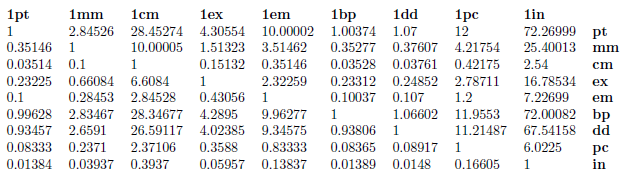
\includegraphics[scale=0.75]{dimentionLatex}
	\caption{Dimension in \LaTeX{}} \label{fig:dimentionLatex}
\end{figure}

\section{Special Characters}

Bear in mind that certain characters are special \LaTeX{} symbols and need to be escaped, as shown in Table~\ref{tab:special:char}.

\begin{table}[htb!]
\caption{Special Characters in \LaTeX}\label{tab:special:char}
\centering
\begin{singlespace}\begin{tabular}{|c | l | l|}
\hline
Symbol & Name & Escape code \\\hline\hline
\# & \normalsize{hash, pound} & \verb|\#| \\
\$ & \normalsize{dollar} & \verb|\$| \\
\% & \normalsize{percent} & \verb|\%| \\
\^{} & \normalsize{``hat''} & \verb|\^{}| \\
\& & \normalsize{ampersand} & \verb|\&| \\
\_ & \normalsize{underscore} & \verb|\_| \\
\{ & \normalsize{left brace} & \verb|\{| \\
\} & \normalsize{right brace} & \verb|\}| \\
\~{} & \normalsize{tilde} & \verb|\~{}| \\
$\sim$ & \normalsize{wide tilde} & \verb|$\sim$| \\
`` & \normalsize{open double quotes} & \verb|``| \\
'' & \normalsize{close double quotes} & \verb|''| \\
\hline
\end{tabular}\end{singlespace}
\end{table}

Note that for quotation marks, you might prefer \verb|``this'' and `that'|  (``this'' and `that')
instead of \verb|"this" and 'that'|  ("this" and 'that'). The symbol \verb|`| can be found below \verb|esc| keyboard, together with tilde \verb|~| symbol. 

If you need to typeset special characters (such as $\curvearrowright$, etc), take a look at the left side on the navigation panel of the TeXstudio. If you installed MiKTeX on a Windows machine, Comprehensive \LaTeX\ Symbol List  could be found under \path|C:\Program Files\MiKTeX 2.9\doc\info\symbols\comprehensive\symbols-a4.pdf|. 


\section{Useful Resources}\label{sec:resources}
\citet{latex:companion} is a \emph{very} useful book --- but it's quite an investment at RM180++.  A worthy one, nevertheless.  \citet{roberts} has a website with very good \LaTeX{} tutorials at \url{http://www.comp.leeds.ac.uk/andyr/misc/latex/}, too.  Don't forget the famous \texttt{lshort} \url{https://tobi.oetiker.ch/lshort/lshort.pdf} tutorial \citep{lshort}. 

You can also find the list compiled by Lim Lian Tze (the template owner of \verb|usmthesis.cls|, which this thesis is based on) at \href{http://liantze.penguinattack.org/latextypesetting}{\texttt{http://liantze.penguinattack.org/latextypesetting}} \citep{lim:latextypesetting}. Also, on my website \href{http://mohdhanafi.unimap.edu.my/template}{\texttt{http://mohdhanafi.unimap.edu.my/}}\citep{matsom:template}.

\section{Useful Tips} %https://www.mackichan.com/index.html?techtalk/395.htm~mainFrame
You might encounter where the section heading in the table of contents appear at the bottom of the page. You can force a page break before a table of content entry. Place an insertion point above the heading in the document, then type \verb|\addtocontents{toc}{\protect\pagebreak}|. Recompile the document and you can see the change on the table of contents.

\noindent For example, the Chapter 3 header appear at the bottom of the page. 

\begin{lstlisting}
	\addtocontents{toc}{\protect\pagebreak}
	\chapter{Figures, Tables, Equations, Algorithms, etc}\label{chap:design}
\end{lstlisting}

If you encounter problems, please make use of google. Start by searching \verb|latex yourproblem|. For example, \verb|latex figure size|. 
	
\chapter{Literature Review}\label{chap:review}

\section{Citations and Bibliography}
This is supposed to be your literature review chapter. Instead, we look at ways to prepare the bibliography and citations instead. 

\section{The \texttt{*.bib} File}
First of all, bear in mind that your bibliography file (\verb|*.bib| files) is like a database like Mendeley.  That means you can maintain a centralised list, and reuse it for all your publications.  \LaTeX{} will only list sources that you actually cite in the text for each document, according to the bibliography and citation style you select in each document.  But you can still hack it so that your own publications are listed, even if you did not cite it. The order of the entry is not important. 
 

\begin{figure}[htb!]
\begin{lstlisting}[language={}]
@BOOK{latex:companion,
  title = {The {\LaTeX} Companion},
  publisher = {Addison-Wesley},
  year = {2004},
  author = {Frank Mittelbach and Michel Goosens and Johannes Braams and David Carlisle and Chris Rowley},
  series = {Addison-Wesley Series on Tools and Techniques for Computer Typesetting},
  address = {Boston, MA, USA},
  edition = {2nd}
}
\end{lstlisting}
\caption{A BibTeX Entry}\label{fig:bibtex}
\end{figure}

\clearpage	% I forced the next paragraph into new page
As an example, in \verb|mybib.bib| I created a Bib\TeX{} entry with JabRef and google scholar, the source text of which is shown in Figure~\ref{fig:bibtex}. Go to \url{https://scholar.google.com/}, click setting (on the left side of the page with three lines), click \verb|Show links to import citations into BibTeX| under the \verb|Bibliography manager| menu, and click \verb|Save|. 

\begin{figure}[htb!]\centering
	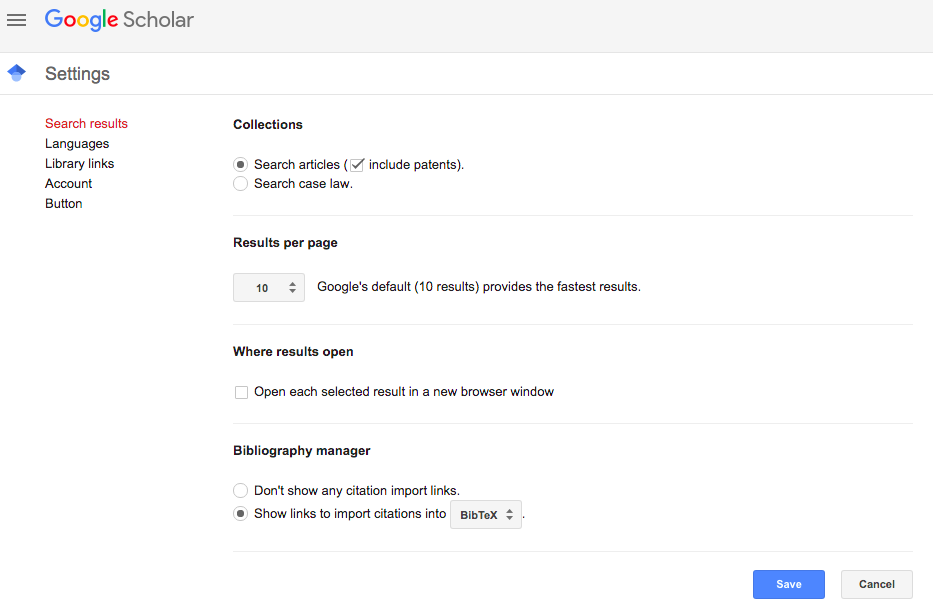
\includegraphics[scale=0.3]{googlescholar}
	\caption{Setting Google Scholar to show Import to BibTeX menu}\label{fig:googlescholar}
\end{figure}

One thing to note about authors' names: Bib\TeX{} recognises ``Mittelbach'' as the last name for both \texttt{Frank Mittelbach} and \texttt{Mittelbach, Frank}.  So for a name like ``Mohd Hanafi Mat Som'' and ``Lim Lian Tze'', you would have to specify it as \texttt{Mat Som, Mohd Hanafi} and either \texttt{Lian Tze Lim} or \texttt{Lim, Lian Tze} for Bib\TeX{} to recognise ``Mat Som'' and ``Lim'' as the last name correctly.  In addition, note that my surname (or family name) consists of multiple words, thus enclose it with braces to avoid surprises, like so: \texttt{Mohd Hanafi \{Mat Som\}}.

\section{Citations using the \texttt{natbib} package}
The \verb|unimapcgsfyp| class imports the \verb|natbib| package which provides citation mechanism as per required by the CGS (and School), so see its documentation for more details.  On a MiK\TeX{} installation,
% it should be in \url{texmf/doc/latex/natbib/natbib.dvi} or \url{natbib.pdf}, in the path where you installed MiKTeX. 
use the command prompt to issue \lstinline|mthelp --view natbib| to access the documentation.
On TeXLive, simply type \verb|texdoc natbib| and the documentation will be displayed automatically, if it's found on your machine.

The basic citation commands are \verb|\citet| and \verb|\citep|, which stands for \emph{textual} and \emph{parenthetical} citation respectively.  They take extra arguments, too, for adding notes in the citations.  Please refer to the \verb|natbib| manual \url{http://texdoc.net/texmf-dist/doc/latex/natbib/natbib.pdf} \cite{cgs:thesis:guideline:2017,latex:companion,lim:2007,lim:latextypesetting}. 

\subsection{IEEE Citation Style}
The default for FYP bibliography style is IEEE:

\begin{itemize}[nosep]\singlespacing
	\item \verb|\citet{latex:companion}| $\to$ \citet{latex:companion}
	\item \verb|\citep{latex:companion}| $\to$ \citep{latex:companion}
	\item \verb|\citet{latex:companion,roberts}| $\to$ \citet{latex:companion,roberts}
	\item \verb|\citep{latex:companion,roberts}| $\to$ \citep{latex:companion,roberts}
	\item \verb|\citet[chap.~2]{latex:companion}| $\to$ \citet[chap.~2]{latex:companion}
	\item \verb|\citep[chap.~2]{latex:companion}| $\to$ \citep[chap.~2]{latex:companion}
\end{itemize}

You may also want to write only the author's name or year occassionally:

\begin{itemize}[nosep]\singlespacing
	\item \verb|\citeauthor{latex:companion}| $\to$ \citeauthor{latex:companion}
	\item \verb|\citeyear{latex:companion}| $\to$ \citeyear{latex:companion}
\end{itemize} 

\subsubsection{Change citation format}

You may want to change the citation format for example in literature review table. See Table~\ref{tab:longtable} in Chapter~\ref{chap:methodology}. This can be achieved using \verb|\setcitestyle{authoryear,round}|. For more information please see the \verb|natbib| documentation. 

\begin{itemize}[nosep]\singlespacing
	\item \verb|\citet{latex:companion}| \\ $\to$ \citet{latex:companion}
	\item { \setcitestyle{authoryear,round} \verb|\citet{latex:companion} {\setcitestyle{authoryear,round} }| \\ $\to$ \citet{latex:companion} } 
	\item \verb|\citet{latex:companion}| \\ $\to$ \citet{latex:companion}
\end{itemize}

\subsection{Entry Types}

This section give some examples of entry of references. There references are formatted according to IEEE style \citep{ieee}. 

\begin{itemize}[nosep]\singlespacing
	\item Journal (\verb|@article|): \citet{othman2019effect} 
	\item Proceeding/Conference (\verb|@inproceedings|): \citet{wanna2018fracture} found that... 
	\item Book (\verb|@book|): As mentioned earlier \citep{latex:companion} 
	\item Internet Sources (\verb|@misc|): As mentioned earlier \citep{lim:latextypesetting} 
\end{itemize}
%\addtocontents{toc}{\protect\pagebreak}
\chapter{Figures, Tables, Equations, Algorithms, etc}\label{chap:design}

%Your chapter.  I probably should include some examples on inserting figures, tables, mathematical equations, etc.

(This is supposed to be the design or methodology chapter.  Instead, we include examples on inserting figures, tables, mathematical equations\ldots i.e.\ things that you might want to include in your thesis.)

\section{Inserting Figures}\label{sec:figure}

You can draw diagrams with special \LaTeX\ commands, but this may take some extra time to learn.  I've had some forays into the \texttt{pgf} and \texttt{tikz} packages and must say I quite like the results; but as I said, they take time to learn. If you want a faster solution, you can draw your diagrams using other applications, and saving them as graphic files (EPS, PNG, JPG, PDF).  

\LaTeX{} requires EPS (encapsulated postscript) graphic files when generating DVI output, and PNG, JPG or PDF when generating PDF output.

For exporting to EPS, try \url{http://www.cloudconvert.com}. It's like a Swiss knife for converting from almost any format, to almost any format.

Here's how to insert a picture with the filename \verb|pythag.eps| or \verb|pythag.png|.  I'm going to display it here with 5cm width, and the caption ``Pythagoras' Theorem''.

\begin{figure}[hbt!]
\begin{lstlisting}
\begin{figure}[hbt!]\centering
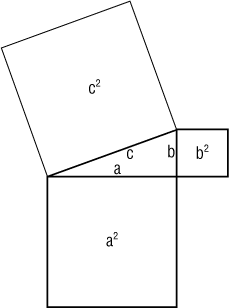
\includegraphics[width=50mm]{pythag}
\caption{Pythagoras' Theorem}
\label{fig:pythagoras}
\end{figure}
\end{lstlisting}
\caption{Including a Graphics File}\label{fig:lst:graphics}
\end{figure}

The result would be:

\begin{figure}[hbt!]\centering
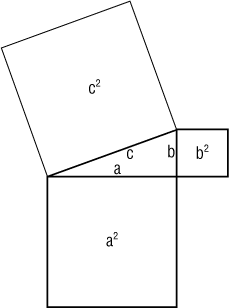
\includegraphics[width=50mm]{pythag}
\caption{Pythagoras' Theroem} \label{fig:pythagoras}
\end{figure}

Don't specify the extension of the graphic file.  The template will automatically look for the EPS or the PNG (or otherwise) versions, depending on whether \verb|latex| or \verb|pdflatex| was used.  The \texttt{figure} environment will also ensure that that an entry is inserted into the \emph{List of Figures} automatically -- including the figure numbering, caption and page number.

In addition, the width of the included graphics can also be specified as a percentage of the text width, e.g.~ \verb|width=.2\textwidth| would cause the graphics to occupy 20\% of the text width.

Notice that I inserted a \verb|\label| just after the \verb|\caption|.  This can be used for referencing the figure number, like this: \\
\verb|Figure \ref{fig:pythagoras}| $\to$ Figure \ref{fig:pythagoras}

This works the same for chapters, sections, tables, equations too.  In \verb|chap-intro.tex|, I labelled the Introduction chapter with \verb|\label{chap:intro}|.  I also labelled the section on inserting figures, \verb|\label{sec:figure}|.  So now I can do \\
\verb|Chapter \ref{chap:intro}| $\to$  Chapter \ref{chap:intro} \\
\verb|section \ref{sec:figure}| $\to$  section \ref{sec:figure}

Everytime the numbering of the heading changes, the reference will change automatically as well.  \textbf{This is another advantage of using \LaTeX{}}: you do not need to manually update the reference counters (nor the Table of Contents, List of Figures and Tables) whenever you add or remove figures, tables, sections or chapters.

You might also want to try out \texttt{Inkscape} or \texttt{FlowframTk}. Both program are a vector graphics and drawing application, and can export to \LaTeX{} code which you can paste into your \LaTeX{} source. \texttt{Inkscape} and \texttt{FlowframTk} are available from \url{https://inkscape.org/} and \url{https://www.dickimaw-books.com/software/flowframtk/}.

\section{How Do I Do Subfigures?}
Here's an example on how to do subfigures (and similarly subtables):

\begin{figure}[hbt!]
\begin{lstlisting}
\begin{figure}[hbt!]
  \begin{minipage}{.49\textwidth}
  \centering
  \subfloat[First caption]{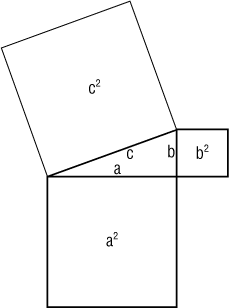
\includegraphics[width=3cm]{pythag}} \label{fig:sub1}
  \end{minipage}
  \hfill
  \begin{minipage}{.49\textwidth}
  \subfloat[Second caption]{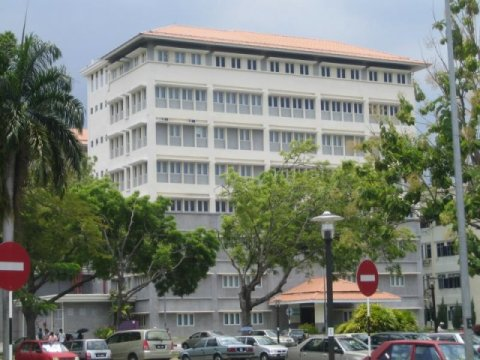
\includegraphics[width=0.8\textwidth]{USMScience}}\label{fig:sub2}
  \end{minipage}
  
  \caption{This is the main caption of the figure.}
  \label{fig:main}
\end{figure}
\end{lstlisting}
\caption{Creating subfigures within figures}
\end{figure}

\begin{figure}[hbt!]
  \begin{minipage}{.49\textwidth}
  \centering
  \subfloat[First caption]{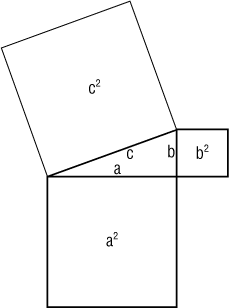
\includegraphics[width=3cm]{pythag}} \label{fig:sub1}
  \end{minipage}
  \hfill
  \begin{minipage}{.49\textwidth}
  \subfloat[Second caption]{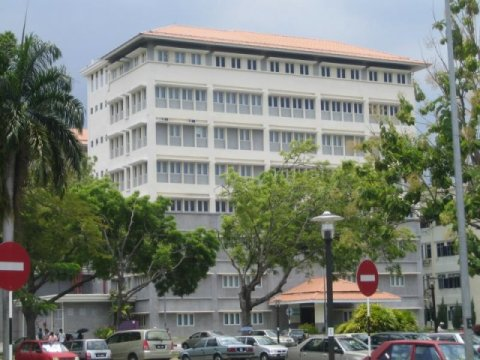
\includegraphics[width=0.8\textwidth]{USMScience}}\label{fig:sub2}
  \end{minipage}
  
  \caption{This is the main caption of the figure.}
  \label{fig:main}
\end{figure}

\section{Inserting Tables}

Typesetting tables can be a little troublesome especially with complex layouts.  Look up \citet{roberts} to learn about some tips, or you can use the online \LaTeX{} table generator (\url{https://www.tablesgenerator.com/}) to help you.

When you're done designing the table, copy the whole table as \LaTeX\ code, and paste it in your source file.  (You may add additional formatting commands, like bold, italics, etc.)  If this is going to be a numbered table, remember to surround it with \verb|\begin{table}| and \verb|\end{table}|, and give it a caption, like this:

\begin{figure}[hbt!]
\begin{lstlisting}
\begin{table}[hbt!]\centering
\begin{tabular}{| l | c || r |}
\hline
\textbf{Name} & \textbf{Category} & \textbf{Quantity} \\ 
\hline\hline
Apple & Fruit & 10 \\ 
\hline
Cucumber & Vegetable & 25 \\ 
\hline
Daisy & Flower & 5 \\ 
\hline
\end{tabular}
\caption{Sample Table Only} \label{table:sample}
\end{table}
\end{lstlisting}
\caption{Typesetting Tables}\label{fig:lst:table}
\end{figure}

\begin{table}[hbt!]\centering
\begin{tabular}{| l | c || r |}
\hline
\textbf{Name} & \textbf{Category} & \textbf{Quantity} \\ 
\hline\hline
Apple & Fruit & 10 \\ 
\hline
Cucumber & Vegetable & 25 \\ 
\hline
Daisy & Flower & 5 \\ 
\hline
\end{tabular}
\caption{Sample Table Only} \label{table:sample}
\end{table}

Note also that \verb|unimapcgsfyp| is configured such that captions for figures are placed \emph{below} the figures, and captions for tables are placed \emph{above} them, in accordance with the formatting guidelines.

Many of us would have had massive headaches about lining up decimal places in table columns if not for this tip from \citet[pp.~274--276]{latex:companion}. This method uses the \verb|dcolumn| package (already loaded by \verb|unimapcgsfyp.cls|). Instead of using \verb|L,C| or \verb|R| as the column type in the \verb|tabulary| declaration, use\\ \texttt{D\{\textit{input sep}\}\{\textit{output sep}\}\{\textit{decimal places}\}}. Note that in Table~\ref{tab:align:decimal}, I use \verb|tabulary| instead of \verb|tabular|. The \verb|tabulary| package is awesome. The column width is set automatically so that it will wrap long sentences into a few lines as demonstrated in Table~\ref{tab:tabletabulary}. 

\begin{figure}[htb!]
\begin{lstlisting}
\begin{table}[htb!]\centering
\begin{tabulary}{\textwidth}{| C | D{.}{.}{3} |}
\hline
Item & \multicolumn{1}{c|}{Reading}\\\hline
A & 1.11\\\hline
B & 3.99\\\hline
C & 2.27\\\hline
\end{tabulary}
\caption{A table with decimal data}
\end{table}
\end{lstlisting}
\caption{Aligning decimal data in tables}\label{fig:align:decimal}
\end{figure}

The \LaTeX\ code in Figure~\ref{fig:align:decimal} will give you Table~\ref{tab:align:decimal}.

\begin{table}[htb!]\centering
\begin{tabulary}{\textwidth}{| C | D{.}{.}{3} |}
\hline
Item & \multicolumn{1}{c|}{Reading}\\\hline
A & 1.11\\\hline
B & 3.999\\\hline
C & 22.2\\\hline
\end{tabulary}
\caption{A table with decimal data}\label{tab:align:decimal}
\end{table}

Without using \verb|dcolumn|, you'd get something like this:

\begin{table}[htb!]\centering
\begin{tabulary}{\textwidth}{| C | R |}
\hline
Item & \multicolumn{1}{c|}{Reading}\\\hline
A & 1.11\\\hline
B & 3.999\\\hline
C & 22.2\\\hline
\end{tabulary}
\caption{A table with decimal data (mis-aligned)}
\end{table}

\begin{table}[H]\singlespacing
	\caption{This is an example to for a table. This is straightforward version.}	\label{tab:tabletabulary}
	\begin{tabulary}{\textwidth}{L R C}
		\toprule[1.5pt]
		Short sentences & short one  & Long sentences \\ \midrule
		This is short.       & 173 & This is much loooooooonger, because there are many more words.  \\ 
		This is not shorter. & put some word here & This is still loooooooonger, because there are many more words. This table make use of \texttt{tabulary} package. \\ \bottomrule[1.5pt]
	\end{tabulary} 
\end{table}

In Table~\ref{tab:tabletabulary} and \ref{tab:tablemulticolumnrow}, I specify the position of the table as \verb|H| instead of \verb|tbh!| so that the table will appear \textbf{HERE} instead of giving the decision to \LaTeX\ for placing the table either \emph{top}, \emph{bottom}, or \emph{here}. 

\begin{figure}[tbh!]
	\begin{lstlisting}
		\begin{table}[H]\centering \singlespacing
		\caption{This is another example for a table. Advance version of a table.}	\label{tab:tablemulticolumnrow}
		\begin{tabulary}{0.8\textwidth}{|C|R|C|}
		\hline
		\multicolumn{2}{|c|}{\textbf{Merge 2 columns}} & \textbf{Long sentences} \\ \hline
		\multirow{2}{=}[-4.5mm]{This is short text LoL.} & \multicolumn{1}{c|}{\multirow{2}{*}{173}} & This is much loooooooonger, because there are many more words.  \\ \cline{2-3}
		& put some word here & This is still loooooooonger, because there are many more words. \\ \hline
		\end{tabulary} 
		\end{table} 
	\end{lstlisting}
	\caption{Note the differences between this table and previous tables.}
\end{figure}

\begin{table}[H]\centering \singlespacing
	\caption{This is another example for a table. Advance version of a table.}	\label{tab:tablemulticolumnrow}
	\begin{tabulary}{0.8\textwidth}{|C|R|C|}
		\hline
		\multicolumn{2}{|c|}{\textbf{Merge 2 columns}} & \textbf{Long sentences} \\ \hline
		\multirow{2}{=}[-4.5mm]{This is short text LoL.} & \multicolumn{1}{c|}{\multirow{2}{*}{173}} & This is much loooooooonger, because there are many more words.  \\ \cline{2-3}
		& put some word here & This is still loooooooonger, because there are many more words. \\ \hline
	\end{tabulary} 
\end{table} 

Table~\ref{tab:tablemulticolumnrow} set the table width so that it will occupy 80\% of the paper width. Then, I use \verb|multirow| package to span through 2 columns. This package also can be made to adjust the vertical alignment in a table whenever a row occupy more than a single line of sentence. \verb|multicolumn| not only use to merge two or more column, but can also be used to change a properties of a single row and column such as the text alignment and table border. 

\begin{table}[H]\centering\singlespacing
	\caption{This is an example to for a table}	\label{tab:tablemulticolumn}
	\begin{tabular}{|l|r|p{7cm}|}
		\hline
		\multicolumn{2}{|c|}{\textbf{Merge 2 columns}} & \textbf{Long sentences} \\ \hline
		\multirow{2}{*}[-4mm]{This is short.} & \multicolumn{1}{c|}{173} & This is much loooooooonger, because there are many more words.  \\ \cline{2-3}
		 & put some word here & This is still loooooooonger, because there are many more words. \\ \hline
	\end{tabular} 
\end{table} 

If you want to specify the exact size of each column, then make use of \verb|p{size}|, \verb|m{size}|, or \verb|b{size}|. \texttt{p} means normal cells, they are like parbox with alignment at the top line. \texttt{b} means alignment at the bottom, so the baseline is at the bottom line. \texttt{m} means alignment in the vertical center, i.e. the baseline is in the center. However, they not work very well with \verb|multitrow|. 

\section{Full-paged, Sideways Figures and Tables}

To make a figure appear on a landscape, full-page layout, put your \verb|\includegraphics| command in a \verb|sidewaysfigure| environment (Figure~\ref{fig:lst:sidewayfigure}).

\begin{figure}[htb!]
\begin{lstlisting}
\begin{sidewaysfigure}\centering
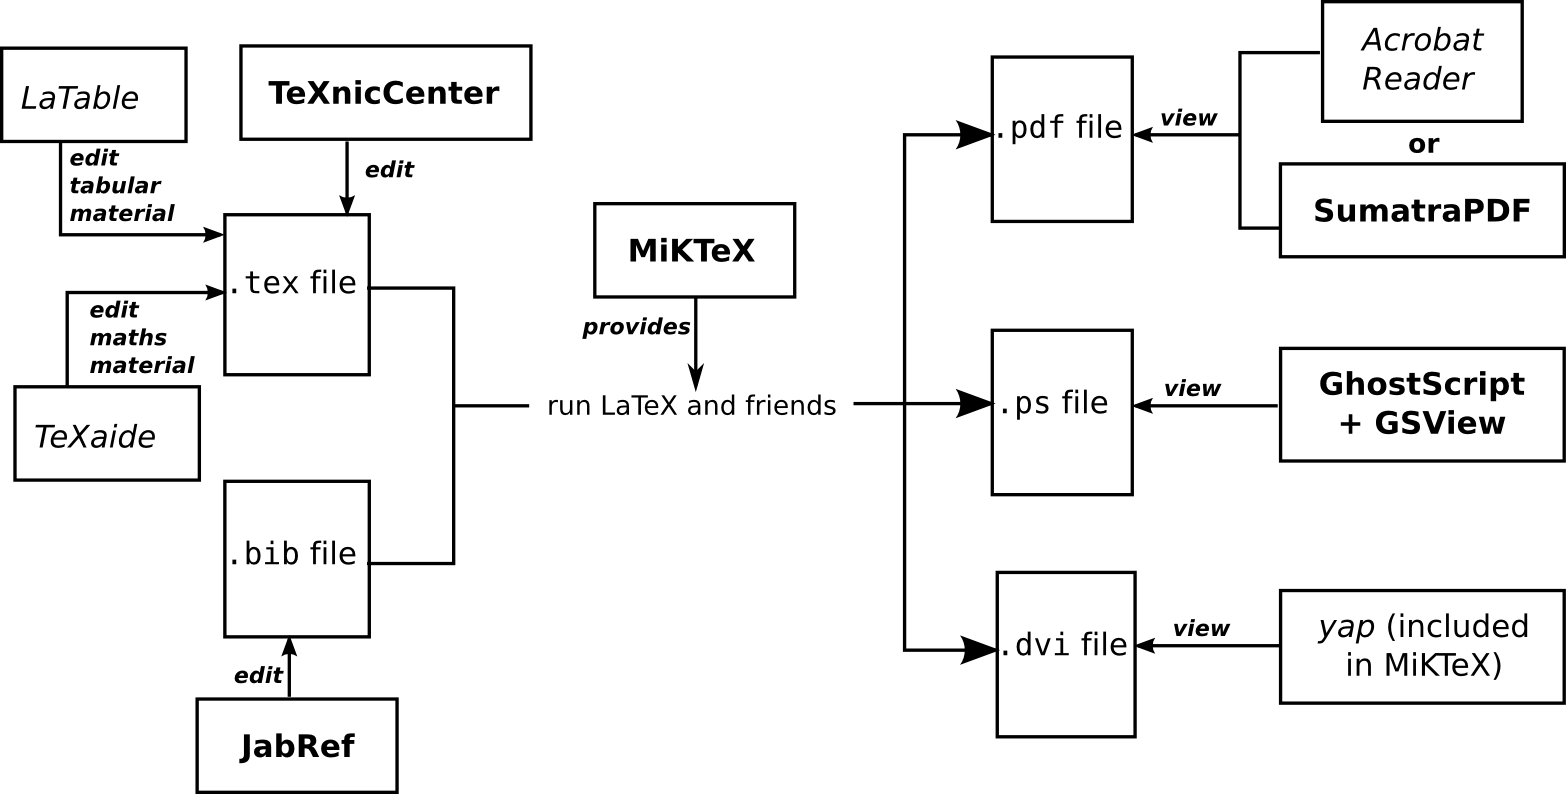
\includegraphics[width=\textheight]{latex-win-comp}
\caption{A full-page, sideways figure}\label{fig:sidewaysfig}
\end{sidewaysfigure}
\end{lstlisting}
\caption{Including a sideway, full-page graphic}\label{fig:lst:sidewayfigure}
\end{figure}

\begin{sidewaysfigure}
\centering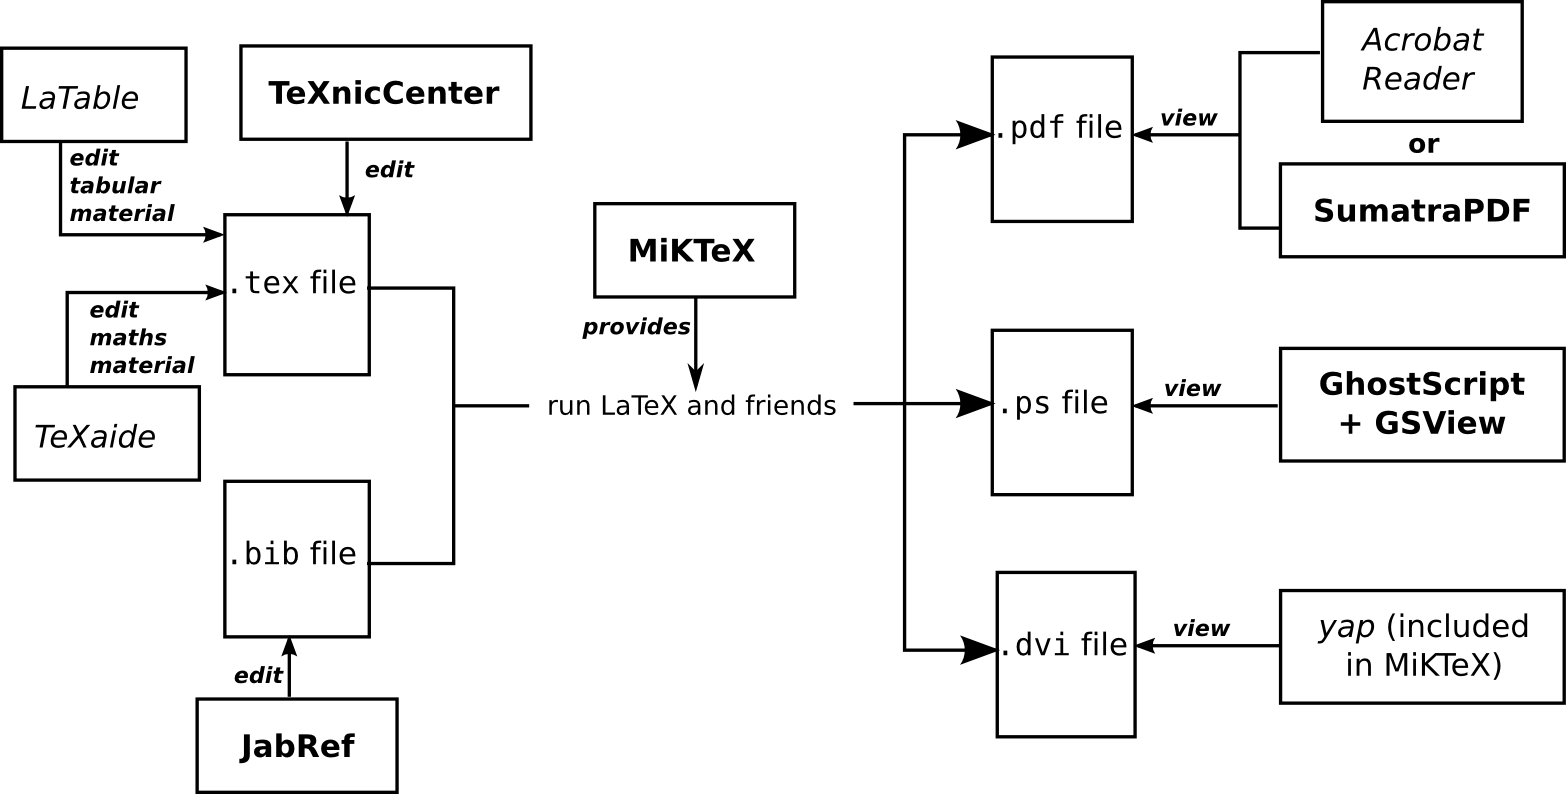
\includegraphics[width=\textheight]{latex-win-comp}
\caption{A full-page, sideways figure}\label{fig:sidewaysfig}
\end{sidewaysfigure}

The resultant figure (Figure~\ref{fig:sidewaysfig}) should appear on the next page.

\begingroup
\setlength{\rotFPtop}{1pc} %
\begin{sidewaystable}
	\singlespacing
		\caption{This is an example to for a table. This is straightforward version.}	\label{tab:sidetabletabulary}
		\begin{tabulary}{\textwidth}{L R C}
			\toprule[1.5pt]
			Short sentences & short one  & Long sentences \\ \midrule
			This is short.       & 173 & This is much loooooooonger, because there are many more words.  \\ 
			This is not shorter. & put some word here & This is still loooooooonger, because there are many more words. This table make use of \texttt{tabulary} package. \\ \bottomrule[1.5pt]
		\end{tabulary} 
\end{sidewaystable}
\endgroup

For a sideways table, use the \verb|sidewaystable| environment instead around your usual \verb|tabular| material. The default positioning of the figure/table is in the middle of a page. You can use \verb|\setlength{\rotFPtop}{1pc}| before the \verb|sidewaystable| environment to change the figure/table positioning. Please enclose the \verb|sidewaystable| environment inside \verb|begingroup| and \verb|endgroup| so that it won't affect the positioning of the figure/table of the whole document. Play around with the size, 1pc, 0pt etc. 

\section{Mathematical Equations}

%Oooh I love this one.  After all, maths is the reason why Donald Knuth created \TeX{}!  It would be quite impossible for me to list all the commands, so I'll just give some example here, and you're better off looking at the various online tutorials like \cite{roberts}.  And TeXnicCenter certainly makes things much easier.

Typesetting mathematical material is one of, if not \emph{the}, strongest capabilities of \LaTeX.  After all, that was the Knuth's main motivation for creating \TeX{}.  As it is impossible to enumerate all possible mathematically-related commands and macros here, we will just give some examples.  The reader is directed to the many well-written online tutorials, such as \citet{roberts}, for more elaborate examples.  TeXnicCenter also provides many shortcut buttons for inserting mathematical symbols.

\begin{figure}[htb!]
\begin{lstlisting}
\begin{equation}\label{eq:pythagoras}
z^2 = x^2 + y^2
\end{equation}

\begin{equation}\label{eq:golden:ratio}
\phi = \frac{1}{2} (1 + \sqrt{5})
\end{equation}

\begin{equation}\label{eq:golden:ratio}
\phi = \frac{1}{2} (1 + \sqrt{5})
\end{equation}
\begin{equation}\label{eq:golden:ratio:fibonacci}
\phi = 1 + \sum ^ {\infty} _ {n=1}
                \frac{ (-1) ^ {n+1} }{ F_n F_{n+1} }
\end{equation}

Equation~\ref{eq:pythagoras} is the Pythagoras Theorem. 
\eqref{eq:golden:ratio} gives the golden ratio $\phi$, and 
\eqref{eq:golden:ratio:fibonacci} relates it to the Fibonacci 
series.
\end{lstlisting}
\caption{Typesetting Mathematical Equations}\label{fig:lst:equation}
\end{figure}

\begin{equation}\label{eq:pythagoras}
z^2 = x^2 + y^2
\end{equation}
\begin{equation}\label{eq:golden:ratio}
\phi = \frac{1}{2} (1 + \sqrt{5})
\end{equation}
\begin{equation}\label{eq:golden:ratio:fibonacci}
\phi = 1 + \sum ^ {\infty} _ {n=1}
                \frac{ (-1) ^ {n+1} }{ F_n F_{n+1} }
\end{equation}

Equation~\ref{eq:pythagoras} is the Pythagoras Theorem. \eqref{eq:golden:ratio} gives the golden ratio $\phi$, and \eqref{eq:golden:ratio:fibonacci} relates it to the Fibonacci series.

The \LaTeX\ code to generate the above mathematics materials are shown in Figure~\ref{fig:lst:equation}.  As you can see, references to equations can be achieved with either \verb|\ref| or \verb|\eqref|. 

You might want to try the online equation edit \url{https://www.mathcha.io/} or \url{https://www.latex4technics.com/} to familiarize with the \LaTeX\ equation. 

\section{Acronyms}
\acresetall
If you have a list of acronyms or symbols, edit the file \verb|loa.tex| as in Figure~\ref{fig:acronym}.

\begin{figure}[hbt!]
\begin{lstlisting}
\begin{acronym}[MMMMMM] %% replace 'MMMMMM' with the longest acronym in your list
\acro{CGS}{Centre for Graduate Studies}
\acro{PPKMt}{Pusat Pengajian Kejuruteraan Mekatronik}
\acro{USM}{Universiti Sains Malaysia}
\acro{UniMAP}{Universiti Malaysia Perlis}
\end{acronym}
\end{lstlisting}
\caption{The template \texttt{loa.tex} for acronyms}\label{fig:acronym}
\end{figure}

You can also use this acronym list to help expand it the first time you mention it in your text.  For example, the first time you use \verb|\ac{UniMAP}|, `\ac{UniMAP}' will be the output (without the quotes).  After that, all calls to \verb|\ac{UniMAP}| will give `\ac{UniMAP}' (without the quotes).  For more information, see the documentation for the \texttt{acronym} package.

\section{Program Listings}

You may have noticed that I used the \verb|lstlisting| environment to typeset some of the \LaTeX{} examples -- with pretty-printing\footnote{Whether you agree that it \emph{is} pretty is another story altogether.}, too, including automatic line-breaking.  For more information, see the documentation for the \verb|listings| package: it's available online at \url{http://www.texdoc.net/pkg/listings}.

Just to give some simple example here.  For example, to typeset a ``Hello World'' Java program with syntax highlighting, you can use the following code:

\begin{figure}[hbt!]
\begin{lstlisting}[escapechar=:,language={}]
\lstset{basicstyle=\small\ttfamily, language=Java, breaklines=true, columns=fullflexible, tabsize=2}
\begin{lstlisting}
public class HelloWorld {
	public static void main( String arg[] ) {
        for (int i = 0; i < 10; i++) {
			System.out.println( "Hello World!" + i);
		}
	}
}
\end:\{:lstlisting:\}:
\end{lstlisting}
\caption{Typesetting a Java program listing}\label{fig:lst:syntax}
\end{figure}

\lstset{keywordstyle={\bfseries}}
\begin{figure}[hbt!]
\lstset{basicstyle=\small\ttfamily, language=Java, breaklines=true, columns=fullflexible, framesep=10pt, xleftmargin=16pt, tabsize=2}
\begin{lstlisting}
public class HelloWorld {
	public static void main( String arg[] ) {
        for (int i = 0; i < 10; i++) {
			System.out.println( "Hello World!" + i);
		}
	}
}
\end{lstlisting}
\caption{A pretty-printed Java program listing with syntax highlighting}
\end{figure}


If you want to turn off the syntax highlighting, set \verb|language={}|.  (See the \verb|listings| documentation for a list of programming languages for which syntax highlighting is supported.)  You can also change the \verb|basicstyle| value to get different effects: e.g. a different font family, size or text formatting.

Here's another example for a C program:

\begin{figure}[hbt!]
\begin{lstlisting}[escapechar={:}, texcl=false,language={}]
\lstset{basicstyle=\sffamily, language=C, breaklines=true, columns=fullflexible, tabsize=2}
\begin{lstlisting}
int main() {
	int c = 0;
	c = c + 1;
	printf( "%d", c );
	return 0;
}
\end:\{:lstlisting:\}:
\end{lstlisting}
\caption{Typesetting a C program listing}\label{fig:lst:c}
\end{figure}

\begin{figure}[hbt!]
\lstset{basicstyle=\sffamily, language=C, breaklines=true, columns=fullflexible, framesep=10pt, xleftmargin=.4\textwidth, tabsize=4}
\begin{lstlisting}
int main() {
	int c = 0;
	c = c + 1;
	printf( "%d", c );
	return 0;
}
\end{lstlisting}
\caption{A pretty-printed C program listing with syntax highlighting}
\end{figure}


And here is the same C program listing \emph{without} syntax highlighting (by setting \verb|language={}|):

\begin{figure}[H]

\lstset{basicstyle=\sffamily, language={}, breaklines=true, columns=fullflexible, framesep=10pt, xleftmargin=.4\textwidth, tabsize=4}
\begin{lstlisting}
int main() {
	int c = 0;
	c = c + 1;
	printf( "%d", c );
	return 0;
}
\end{lstlisting}
\caption{A C program listing without syntax highlighting}
\end{figure}

\chapter{Result \& Discussion}\label{chap:implementation}

Now is the time to ``implement'' your thesis with \LaTeX.  Go forth and typeset! Happy \LaTeX{}ing! %\Smiley

\section{Printing Your Thesis}
This is \emph{very} important. Assuming you're printing your thesis from Acrobat Reader, make sure the following settings are chosen correctly in the Print window:

\begin{itemize}[nosep]
\item A4 paper size is selected.
\item Make sure your Printer settings is using A4 too.
\item No page scaling.
\end{itemize}

Otherwise, the margins of your printed outputs may go horribly wrong. Print one or two pages first to make sure everything looks fine before printing your entire thesis.
%\include{chap-discussion}
\chapter{Conclusion}

T-that's all folks.  Have fun with \LaTeX!. 

%%%%%%%%%%%%%%%%%%%%%%%%%%%%%%%%%%%%%%%%%%%%%%%%%%%%%%%
%TODO Bibliography.
% You can create mybib.bib with JabRef, the program included
% download from
% http://jabref.sourceforge.net/
% \shortcite for APA style https://latex.org/forum/viewtopic.php?f=50&t=22088
%%%%%%%%%%%%%%%%%%%%%%%%%%%%%%%%%%%%%%%%%%%%%%%%%%%%%%%
\titlespacing*{\chapter}{0pt}{*-4.5}{\baselineskip}
\bibliography{IEEEabrv,mybib}
%\printbibliography
	

%%%%%%%%%%%%%%%%%%%%%%%%%%%%%%%%%%%%%%%%%%%%%%%%%%%%%%%
%TODO Appendices.
%%%%%%%%%%%%%%%%%%%%%%%%%%%%%%%%%%%%%%%%%%%%%%%%%%%%%%%
\appendix
\chapter{Data Used}

Put some test data here.
\chapter{UML Diagrams}

Yet another dummy placeholder for appendix material.

\chapter{Dummy Appendix}

%%%%%%%%%%%%%%%%%%%%%%%%%%%%%%%%%%%%%%%%%%%%%%%%%%%%%%%
%TODO List of publication appendix.  If you don't have one, you may
% comment out the next 4 lines.
%%%%%%%%%%%%%%%%%%%%%%%%%%%%%%%%%%%%%%%%%%%%%%%%%%%%%%%
%\nociteown{lim:2007,lim:latextypesetting}
%\begin{singlespace}
%\bibliographyown{mybib}
%\end{singlespace}

\end{document}
